\scanpage{13}

\figure{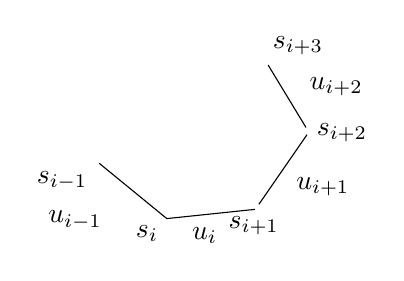
\begin{tikzpicture}[x=.013cm,y=-.013cm]
\draw (102,151)--(168,205)--(254,196);
\draw (258,191)--(305,123); \draw (304,116)--(267,55);
\node[left] at (100,168) {$\unsure{s}_{i-1}$};
\node[below left] at (114,188) {$u_{i-1}$};
\node[below left] at (169,202) {$s_i$};\node[below] at (205,204) {$u_i$};
\node[below] at (253,193) {$s_{i+1}$};\node[right] at (285,174) {$u_{i+1}$};
\node[right] at (305,121) {$s_{i+2}$};\node[right] at (298,76) {$u_{i+2}$};
\node[above right] at (262,55) {$s_{i+3}$};
\end{tikzpicture}}

\[\resizebox{\ifdim\width>\linewidth\linewidth\else\width\fi}{!}{$\displaystyle
\begin{aligned}
 \text{hyp \unsure{de donn.|donn.|données}}\quad&
 \left\{\begin{aligned}u&=\lambda_i u_{i-1}-\lambda_{i+1}u_{i+1}
 \qquad i=0,1,\ldots,n-1\\ \sum u_i&=0\end{aligned}\right.\\
 \text{(\unsure{def|déf})}\quad&
 \left\{\begin{aligned}u_{i-1}\wedge u_i&=\mu_i\\u\wedge u_i&=\alpha_i\end{aligned}\right.
 \quad\deleted{\unsure{\big\}\ (\mathrm{def})}}
\end{aligned}
$}\]
\[
 \deleted{u\ne0\quad
 \left.\begin{gathered}u_i\ne0\\\lambda_i\ne0\end{gathered}\right\}\forall i
 \quad\Longrightarrow(\unsure{\alpha|u_i})_i\ne}
\]
\[\resizebox{\ifdim\width>\linewidth\linewidth\else\width\fi}{!}{$\displaystyle
 \underbrace{\left.\begin{aligned}(\mu_i)_i&\ne0\ -\\
 \text{et }\ u&\ne0\end{aligned}\right\}\Longleftrightarrow(\alpha_i)_i\ne0}_{\text{hyp}}
 \qquad\unsure{\text{et}}\quad
 \underbrace{u_i\ne0,\ \lambda_i\ne0\quad\forall i}_{\text{hyp.}}
$}\]
\[\resizebox{\ifdim\width>\linewidth\linewidth\else\width\fi}{!}{$\displaystyle
 \left\{\begin{aligned}
 \lambda_i\mu_i+\lambda_{i+1}\mu_{i+1}&=\alpha_i\\
 \lambda_i\alpha_{i-1}-\lambda_{i+1}\alpha_{i+1}&=0\\
 \sum\alpha_i&=0\qquad 2\sum\lambda_i\mu_i=0
 \end{aligned}\right.
 \qquad
 \begin{aligned}(\lambda_i,\alpha_i)_i&\ne0\\
 &P(k^n\times L^n)\end{aligned}
$}\]
\deleted{\unsure{($\lambda_i$) connu quand on connaît}}

\[\resizebox{\ifdim\width>\linewidth\linewidth\else\width\fi}{!}{$\displaystyle
\begin{aligned}
 u_0,u_1,u,(\lambda_i)&\Longrightarrow u_i\quad\forall\ \deleted{\unsure{\in}}i\\
 \alpha_0,\alpha_1,(\lambda_{\unsure{0|i}})&
 \underset{\text{si }\mu_1\ne0}{\Longrightarrow}(u_i)\ \text{mod Gp Aff}
\end{aligned}
$}\]
\[\resizebox{\ifdim\width>\linewidth\linewidth\else\width\fi}{!}{$\displaystyle
\begin{aligned}
 &\deleted{\unsure{(\alpha_i),(\lambda_i)}}\\
 u&=\frac{\alpha_1}{\mu_1}u_0-\frac{\alpha_0}{\mu_1}u_1
 =\left(\lambda_1+\lambda_2\frac{\mu_2}{\mu_1}\right)u_0-
 \left(\lambda_0\frac{\mu_0}{\mu_1}+\lambda_1\right)u_1\\
 &(\lambda_i,\deleted{\unsure{\alpha_i}}\mu_i)_i\quad\text{mod }k^\ast\quad .
\end{aligned}
$}\]

$CI_n^\ast={}$ $n$-polygônes critiques (mod Aff) \deleted{\unsure{de qui}} qui ne sont \unsure{en !|pas !} \deleted{\unsure{$\lambda_i\ne0\ \forall i$}} \deleted{\unsure{multi}}triangulaires

\[\resizebox{\ifdim\width>\linewidth\linewidth\else\width\fi}{!}{$\displaystyle
 \begin{aligned} &\big\downarrow\\&P^{n-1}\times P^{n-1}\\
 &(\lambda_i)\qquad(\mu_{\unsure{j|i}})\end{aligned}
 \qquad
 \begin{aligned}
 \deleted{\unsure{\lambda_2}}u_2&=-\deleted{\unsure{\lambda_2}}\frac{\mu_2}{\mu_1}u_0+
 \frac{1}{\lambda_2}\left(\lambda_0\frac{\mu_0}{\mu_1}+\lambda_1\right)u_1\\
 &\cdots\\
 u_{n-1}&=A_{n-1}\bigl((\lambda)(\mu)\bigr)u_0+B_{n-1}(\ ,\ )u_1
 \end{aligned}
$}\]
% archive sheet number: 19
